\label{chp:implementation}

The theoretical background for the \emph{ab initio} simulation of thermal conductivity has been established in the previous chapters, in particular, Chp.~\ref{chp:heat_transport}. The purpose of this chapter is to discuss the practical implementation of the respective formulas for two benchmark materials. The scheme is implemented in FHI-vibes~\cite{FHI-vibes}.

\newthought{We restate the Green-Kubo formula} for the thermal conductivity initially introduced in Sec.\,\ref{sec:ab_initio_heat_flux} as
\begin{align}
	\kappa^{\alpha \beta} (T)
		= \int \d \Gamma_0 ~ \kappa^{\alpha \beta} (\Gamma_0) f_T (\Gamma_0) ~,
	\label{eq:implementation.kappa.avg}
\end{align}
where $\kappa^{\alpha \beta} (T)$ are the Cartesian components of the thermal conductivity tensor at temperature $T$,\footnote{$T$ represents all thermodynamic conditions in the simulation, including pressure $p$.} and $\Gamma_0$ are phase-space configurations with a respective ensemble weight $f_T (\Gamma_0)$ at the given temperature. For each phase-space configuration $\Gamma_0$, the thermal conductivity is computed as
\begin{align}
	\kappa^{\alpha \beta} (\Gamma_0)
		&=
		\frac{V}{k_{\rm B} T^2} 
		\lim_{t_{\rm c} \to \infty}
		\int_{0}^{\tcut} 
		\d t ~ C_{JJ}^{\alpha \beta} (\Gamma_0, t)~.
	\label{eq:implementatino.kappa.1}
\end{align}
Here, $	C^{\alpha \beta}_{J J} (\Gamma_0, t)$ denotes the heat flux autocorrelation function (HFACF),
\begin{align}
	C^{\alpha \beta}_{J J} (\Gamma_0, t)
		=
		\lim_{t_{0} \to \infty}
		\frac{1}{t_0 - t}
		\int_{0}^{t_{\rm 0} - t} 
		\d s ~ J^\alpha (\Gamma_{t + s}) J^\beta (\Gamma_s)~,
	\label{eq:implementatino.acf.1}
\end{align}
which can be viewed as an average over all available starting conditions $\Gamma_s$ during a simulation of length $t_0$. Each phase-space point $\Gamma_t$ is related to the initial configuration $\Gamma_0$ through the canonical time evolution determined by the many-body Hamiltonian of the system, $\mathcal H (\Gamma)$. Equation~\eqref{eq:implementation.kappa.avg} through~\eqref{eq:implementatino.acf.1} represent an exact reformulation of the Green Kubo formula.


\newthought{In order to evaluate these equations in finite simulations}, the integrals need to be discretized and truncated to finite domains. First, we approximate Eq.\,\eqref{eq:implementation.kappa.avg} by choosing a finite set of $M$ starting configurations $\Gamma_0^i$, so that
\begin{align}
	\kappa^{\alpha \beta} (T)
		\approx
		\frac{1}{M} \sum_{i=1}^M \kappa^{\alpha \beta} (\Gamma_0^i)~,
	\label{eq:implementation.kappa.mean}
\end{align}
where the starting conditions $\Gamma_0^i$ are chosen from NVT molecular dynamics simulations for the thermodynamic conditions of interest. For each starting condition $\Gamma_0^i$, we perform NVE molecular dynamics simulations to generate the time evolution of the system, $\Gamma_t^i$, 
%\mscomment{you don't need initial equilibration?}
%\FK{All convergence checks go by discarding the first time period, I didn't see an effect there when discarding a few ps. I think it really depends on the quantity one is interest in. Also it's often a minor error compared to things like energy drift in aiMD runs, I would guess.}
and evaluate the heat flux, $J^\alpha (\Gamma_t^i)$ along this trajectory. The simulation is performed for a total simulation time $t_0$, thereby truncating the time integral in Eq.\,\eqref{eq:implementatino.acf.1}. From the resulting autocorrelation function of finite length, the thermal conductivity is computed via Eq.\,\eqref{eq:implementatino.kappa.1}, where a \emph{cutoff time} $\tcut < t_0$ is chosen to avoid integrating parts of the autocorrelation function after it has effectively decayed, as non-zero values are only due to statistical fluctuations stemming from finite size and time effects~\cite{Jones.2012}.
%\mscomment{what noise?}
%\FK{statistical noise in the ACF due to finite size/finite time scales. Not fully balances statistical distribution of phonon modes, etc}
After computing the thermal conductivity for each trajectory, the final value is given by Eq.\,\eqref{eq:implementation.kappa.mean},~i.\,e.,~by the \emph{mean} of the individual trajectories. The statistical error due to the finite ensemble average is estimated by the \emph{standard error},~i.\,e.,~the standard deviation of the mean,
\begin{align}
	\Delta \kappa^{\alpha \beta} (T)
		= \frac{1}{\sqrt{N}} \sqrt{\frac{1}{N} \sum_i \left( \kappa^{\alpha \beta} (T) - \kappa^{\alpha \beta} (\Gamma_0^i) \right)^2}~.
	\label{eq:imp.kappa.err}
\end{align}
From the Cartesian components of the thermal conductivity $\kappa^{\alpha \beta} (t)$, the scalar thermal conductivity $\kappa (T)$ is obtained via
\begin{align}
	\kappa (T)
		= \frac{1}{3} \sum_{\alpha} \kappa^{\alpha \alpha} (T)~.
	\label{eq:kappa.scalar}
\end{align}


\newthought{In empirical force field approaches}, the appearing equations can be evaluated as is, and convergence in size and time can be checked in a brute-force way by increasing the respective scales well beyond the necessary limits.
%\CITE{Lammps, Jones, more}. 
From an \emph{ab initio} perspective, the accessible size and time scales are each at least two orders of magnitude lower,\footnote{Force fields: 1\,ns for 10000~atoms within 1 day on one supercomputer node, \emph{ab initio}: 50\,ps for 200~atoms within 1~months on five supercomputer nodes.} and additional steps are necessary to increase the amount of information that can be extracted from the comparatively short simulations. The purpose of this chapter is to discuss these additional steps in detail: First, we present steps to remove noise from the heat flux autocorrelation functions $C_{JJ} (t)$, which enables to choose cutoff times $\tcut$ in a numerically robust way. Next, we discuss the size extrapolation scheme in terms of the harmonic mapping presented in Sec.\,\ref{sec:aiGK} which allows to correct for the finite size of simulations cells used in \emph{ab initio} molecular dynamics simulations. Finally, we discuss the necessary simulation times $t_0$ and how those can be estimated for novel materials.

\newthought{We present the implementation in detail} for the case of periclase magnesium oxide (MgO) which is well-known in the literature, and, as a rather harmonic material, a typical benchmark system for perturbative heat transport techniques. We then apply the same approach to the strongly anharmonic marshite copper iodide (CuI), for which basic assumptions of perturbation theory are violated, as we will explain in detail. 
Both structures are studied at GGA level of theory using the PBEsol functional and light-default basissets in FHI-aims~\cite{Perdew.2008,FHI-aims}. Supercell sizes are 216 atoms each, and the MD simulations are performed via FHI-vibes~\cite{Larsen.2017,FHI-vibes}. The aiGK methods as described is implemented in FHI-vibes as well. Force constants for the size extrapolation via harmonic mapping are obtained via regression from the MD runs via the temperature dependent effective potentials code (TDEP)~\cite{Hellman.2013}. The MD runs are thermalized using the pre-thermalization technique outlined in Sec.\,\ref{sec:harmonic_sampling} using finite-differences force constants obtained via phonopy~\cite{phonopy}. Afterwards, a Langevin thermostat at the target temperature (300\,K) is used to perform NVT sampling. After and initial sampling period of 2.5\,ps, the thermal pressure is relaxed according to the scheme outlined in Sec.\,\ref{sec:app.lattice_expansion} in the appendix to account for thermal expansion. Starting points $\Gamma^i_0$ for the NVE simulations are chosen from an NVT run for the relaxed supercell at least 2\,ps apart. The time step for the MD simulation was chosen as 5\,fs, which corresponds to a tenth of the shortest period duration of the harmonic spectrum of MgO ($\omega_{\rm max} \approx 20$\,THz).


\section{Noise Reduction Scheme and Cutoff Estimation}
\subsection{Discard non-contributing terms}
The raw \emph{ab initio} heat flux used in this work was defined in Eq.\,\eqref{eq:J_ai} and is given for a phase-space point $\Gamma_t = \set{{\bf R} (t), \dot{\bf R} (t)}$ by
\begin{align}
	{\bf J}^{\rm raw} (t) 
		= \frac{1}{V} \sum_I \sigma_I (t)  \dot{\bf R}_I (t)~,
	\label{eq:imp.J.0}
\end{align}
where $\sigma_I (t) \equiv \sigma_I [{\bf R} (t)]$ are atomic virial tensors for the configuration at the given time $t$ as defined in Eq.\,\eqref{eq:hf.sigma_I}, and $\dot{\bf R}_I (t)$ is the velocity of atom $I$ as usual. We split the raw flux in two parts,
\begin{align}
	{\bf J}^{\rm raw} (t)
		= \frac{1}{V} \sum_I \delta \sigma_I (t) \dot{\bf R}_I (t) 
		+ \frac{1}{V} \sum_I \braket{\sigma_I} \dot{\bf R}_I (t)~,
	\label{eq:imp.J.1}
\end{align}
where $\braket{\sigma_I}$ is the average atomic virial, and $\delta \sigma_I (t)$ is the time-dependent part. In the absence of diffusion, the second term is the total time derivative of a bounded vector field, $\sum_I \braket{\sigma_I} \dot{\bf R}_I (t) = \frac{\d}{\d t} \sum_I \braket{\sigma_I} {\bf R}_I (t)$. By means of the gauge invariance principle introduced in Sec.\,\ref{sec:gauge_invariance}, it therefore does not contribute to the time integral in Eq.\,\eqref{eq:implementatino.kappa.1}, and can be discarded before evaluating the heat flux autocorrelation function~\cite{Ercole.2016}. We therefore always use the following heat flux expression:
\begin{align}
	{\bf J} (t)
		= \frac{1}{V} \sum_I \delta \sigma_I (t) \dot{\bf R}_I (t)~.
	\label{eq:imp.J}
\end{align}
Depending on the material, discarding the non-contributing part from the raw heat flux reduces the noise in the simulation \emph{massively}, as shown for the case of MgO in the upper panel of Fig.\,\ref{fig:imp.hfacf.kappa.1} (orange curves compared to light blue curves).

Due to the finite time of the simulation, we furthermore enforce a vanishing expectation of the flux to remove bias from the resulting quantities by removing the finite-time average, ${\bf J} (t) \to \delta {\bf J} (t) = {\bf J} (t) - \braket{{\bf J}}_t$.
%
\begin{figure}
	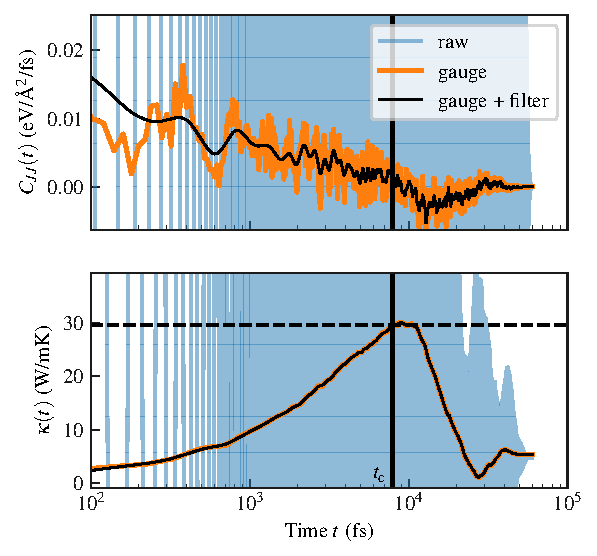
\includegraphics[width=\textwidth]{./data/plots/implementation/MgO/hfacf_data_yy_3.pdf}
	\caption{Heat flux autocorrelation function $C_{JJ}(t)$ (HFACF) as defined in Eq.\,\eqref{eq:implementatino.acf.1} and its cumulative integral,~i.\,e.,~the thermal conductivity $\kappa (t)$ as function of lag time $t$. Light blue: $C_{JJ}(t)$ and $\kappa (t)$ obtained by using the raw flux as defined in Eq.\,\eqref{eq:imp.J.0}. Orange: After discarding the gauge-invariant term in Eq.\,\eqref{eq:imp.J.1}. Black curves: After applying additional, integral-preserving noise filtering as explained in the main text. The cutoff time $t_{\rm c}$ is chosen based on the ``first dip'' of the noise-filtered HFCAF.
	\emph{Computational details:} The shown data is for the $\kappa^{yy}$-component of MgO in an aiMD simulation of 60\,ps total length using a time step of 5\,fs. The heat flux was evaluated every four steps. The system was thermalized to 300\,K using a Langevin thermostat. The system size is 216 atoms in a cubic supercell.}
	\label{fig:imp.hfacf.kappa.1}
\end{figure}

\subsection{Noise filtering}
After discarding the gauge-invariant contributions from the heat flux, there is still a considerable level of noise in the HFACF, which hinders a robust identification of the time at which it is fully decayed,~i.\,e.,~the cutoff time $\tcut$. Available techniques to identify cutoff times, such as the first avalanche method introduced in Ref.\,\cite{Chen.2010}, are not fully parameter-free, and need hand tuning, even if very little.\footnote{The first avalanche technique determines cutoff times by means of a signal-over-noise ratio and relies on two parameters, a window size for computing moving averages, and a threshold value for the resulting avalanche function.} We therefore suggest an approach that does rely only on a single parameter which is chosen based on the vibrational spectrum of the material: Motivated by the fact that the \emph{integrated} HFACF,~i.\,e.,~the cumulative thermal conductivity
\begin{align}
	\kappa (t)
		=
		\frac{V}{k_{\rm B} T^2} 
		\int_{0}^{t} 
		\d t' ~ C_{JJ} (t')~,
	\label{eq:imp.kappa.cum}
\end{align}
is already a much smoother function than the HFACF itself, we apply a shape-preserving Savitzky-Golay filter to $\kappa (t)$ as implemented in Scipy~\cite{Savitzky.1964,scipy}. The remaining parameter is the window size for the filter. It is chosen based on the vibrational spectrum of the material by taking the period length corresponding to the slowest significant frequency $\omega_{\min}$. Thereby, all noise of higher frequency is effectively filtered from $\kappa (t)$, while all relevant time integrals are preserved by construction: The cumulative kappa before (orange curve) and after (black curve) lie right on top of each other in the lower panel of Fig.\,\ref{fig:imp.hfacf.kappa.1}. The filter is constructed such that the antisymmetry of $\kappa (t)$ in time, $\kappa (-t) = - \kappa (t)$ is respected.\footnote{The antisymmetry of $\kappa (t)$ is a consequence of the time symmetry of $C_{JJ} (t)$.} This also ensures that $\kappa (t)$ vanishes identically at $t=0$.

Based on the filtered cumulative thermal conductivity, the HFCAF can be obtained by differentiating, which carries over the filtering to $C_{JJ} (t)$. The filtered HFACF can be obtained analytically by fitting spline functions to $\kappa (t)$, or numerically by applying the same filter on the numerical gradient of $\kappa (t)$. The resulting cumulative thermal conductivity $\kappa (t)$ and HFACF $C_{JJ} (t)$ are shown as black curves in Fig.\,\ref{fig:imp.hfacf.kappa.1}. From the noise-filtered HFACF, the cutoff time $\tcut$ is chosen by a ``first dip'' criterion,~i.\,e.,~when $C_{JJ} (t)$ drops to zero~\cite{Chen.2010}. This corresponds to the first significant plateau in $\kappa (t)$ after removing the noise. With the cutoff time $\tcut$, the resulting thermal conductivity for a given component of the thermal conductivity tensor is given by the value $\kappa = \kappa (\tcut)$ as indicated by the dashed horizontal line in Fig.\,\ref{fig:imp.hfacf.kappa.1}.
The presented scheme will be used for all reported values of thermal conductivity in the following.

\section{Size extrapolation}
\label{sec:imp.extrapolation}

%\mscomment{tell more clearly what is new and what not}
After we have seen how the Green-Kubo formula is used to compute thermal conductivities from the \emph{ab initio} heat flux evaluated along aiMD trajectories, we shortly review the size extrapolation scheme first introduced in Ref.\,\cite{Carbogno.2016} and discussed in more detail in Sec.\,\ref{sec:aiGK}. The aim of the size extrapolation is to correct for finite size effects occuring in aiMD simulations, because the supercells used in \emph{ab initio} simulations are limited in size, and phonon modes of longer wavelength than the supercell are therefore not included. 

\newthought{As discussed in Sec.\,\ref{sec:aiGK}}, the correction works by computing the harmonic contribution to the thermal conductivity $\kappa_{\rm ha}$ within the supercell via Eq.\,\eqref{eq:ha.kappa.bte}
\begin{align}
	\kappa_{\rm ha}^{\alpha \beta} = V k_{\rm B} \sum_{b, {\bf q}} v^\alpha_b ({\bf q}) v^{\beta}_b ({\bf q}) \fD \tau_b ({\bf q})~,
	\label{eq:imp.K.bte}
\end{align}
where $v_b^\alpha ({\bf q})$ is the group velocity of a phonon mode with band index $b$ and \emph{commensurate} wave vector $\bf q$, and $\tau_b ({\bf q})$ is the lifetime obtained from the autocorrelation function of the mode-resolved energy $E_b ({\bf q}, t)$ as defined and discussed in Eq.\,\eqref{eq:G_s}~\cite{Carbogno.2016}. For a given simulation $\set{\Gamma^i  _t}$, Eq.\,\eqref{eq:imp.K.bte} is evaluated for all commensurate $\bf q$-points, and projected to the symmetry-inequivalent points in the Brillouin zone determinded by the space group operations of the system to improve the statistics~\cite{Maradudin.1968}. The irreducible q-points in the Brillouin zone are obtained by iteratively reducing the given grid with the available symmetry operations for the system obtained by the spglib package~\cite{Spglib}.

\newthought{In the next step}, the lifetimes $\tau_b ({\bf q})$ are interpolated to denser $\bf q$-point meshes by $\fD{\tilde{\tau}}_b (\tilde{\bf q}) = \fD \lambda_b (\tilde {\bf q}) \omega_b^{-2} (\tilde {\bf q})$ with a weakly $\bf q$-dependent function $\lambda_b (\tilde {\bf q})$ obtained by linearly interpolating the lifetimes obtained at commensurate $\bf q$-points.\footnote{We use linear interpolation at variance with Ref.\,\cite{Carbogno.2016}, as we found it to be numerically more robust. However, results should not significantly depend on the interpolation algorithm used to obtain $\lambda_b (\tilde {\bf q})$, as the physically relevant contribution is captured by the $\omega_b^{-2} ({\bf q})$  scaling.} The scaling of lifetimes with $\omega_b^{-2} ({\bf q})$ is rooted in basic phonon theory as discussed in detail by Herring~\cite{Herring.1954}. For the acoustic modes at ${\bf q} = \Gamma = 0$, where $\omega ({\bf q \to 0}) \to 0$, the value for $\lambda_b (\Gamma)$ is obtained by averaging over values at the surrounding $\bf q$-points. For the new, denser grid, an interpolated value,
\begin{align}
	\kappa_{\rm ha - int}^{\alpha \beta} (N_{\tilde{\bf q}}) = V k_{\rm B} \frac{N_{\bf q}}{N_{\tilde{\bf q}}} \sum_{b, \tilde{\bf q}} v^\alpha_b (\tilde{\bf q}) v^{\beta}_b (\tilde{\bf q}) \fD{\tilde{\tau}}_b (\tilde{\bf q})~,
	\label{eq:imp.K.bte.correction}
\end{align}
can be obtained, where $N_{\tilde{\bf q}}$ is the number of points in the new grid, and the factor $N_{\bf q} / N_{\tilde{\bf q}}$ accounts for the increased number points. The bulk limit of Eq.\,\eqref{eq:imp.K.bte.correction} is obtained by computing interpolated values for an increasing density of $\bf q$-points. Since Eq.\,\eqref{eq:imp.K.bte.correction} is a Riemann sum approximating the Brillouin zone integral $\int \d^3 q$, its convergence can be expected to be linear in $N_{\tilde{\bf q}}^{-1/3} \equiv 1 / n_q$, where $n_q$ is number of $\bf q$-points per Cartesian direction. The slope of this curve can be used to extrapolate the value of $\kappa_{\rm ha}$ to bulk limit, as shown in Fig.\,\ref{fig:imp.kappa.bte.correction}.
\begin{figure}
	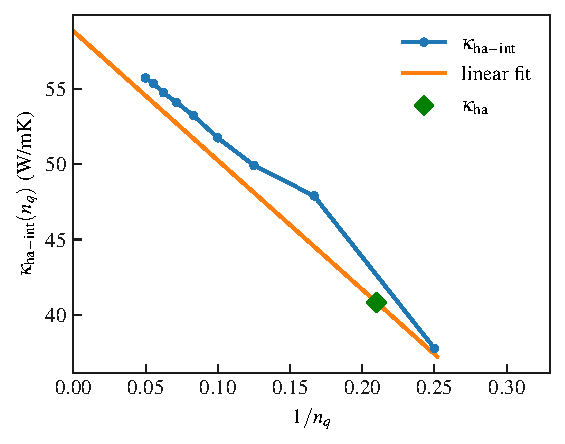
\includegraphics[width=.8\textwidth]{./data/plots/lifetimes/greenkubo_summary_interpolation_fit.pdf}
	\caption{Size extrapolatino correction to bulk limit computed from Eq.\,\eqref{eq:imp.K.bte.correction} assuming linear convergence in $1 / n_q$, where $n_q$ is the number of {\bf q}-points per Cartesian direction.}
	\label{fig:imp.kappa.bte.correction}
\end{figure}
With the extrapolated value $\kappa_{\rm ha-bulk}$, a correction can be obtained via
\begin{align}
	\delta \kappa_{\rm ha-correction} 
		= \kappa_{\rm ha-bulk} - \kappa_{\rm ha}~,
	\label{eq:imp.K.correction}
\end{align}
from which the final result for the thermal conductivity is obtained via
\begin{align}
	\kappa^{\alpha \beta}_{\rm corrected}
		 = \kappa^{\alpha \beta} + \delta \kappa^{\alpha \beta}_{\rm ha-correction}~,
	\label{eq:imp.K.corrected}
\end{align}
where $\kappa^{\alpha \beta}$ is the value from the \emph{ab initio} Green Kubo simulation. The interpolation scheme effectively subtracts harmonic contributions to the thermal conductivity from vibrations commensurate with the supercell, and extrapolates them to the bulk limit, thereby including long-range contributions otherwise not present in the simulation cell.

\section{Simulation Time Convergence}
\label{sec:implementation.convergece}
After we have seen how the cutoff time $\tcut$ in Eq.\,\eqref{eq:implementatino.kappa.1} can be obtained, and finite-size errors can be corrected, we discuss the convergence of presented scheme as a function of the simulation time $t_0$ in Eq.\,\eqref{eq:implementatino.acf.1}. We do this for the case of MgO for three independent trajectories of 60\,ps length each. We truncate every trajectory in 10\,\% steps down to a length of 6\,ps, and apply the workflow presented in the previous sections to each of the truncated trajectories. 
\begin{figure}
	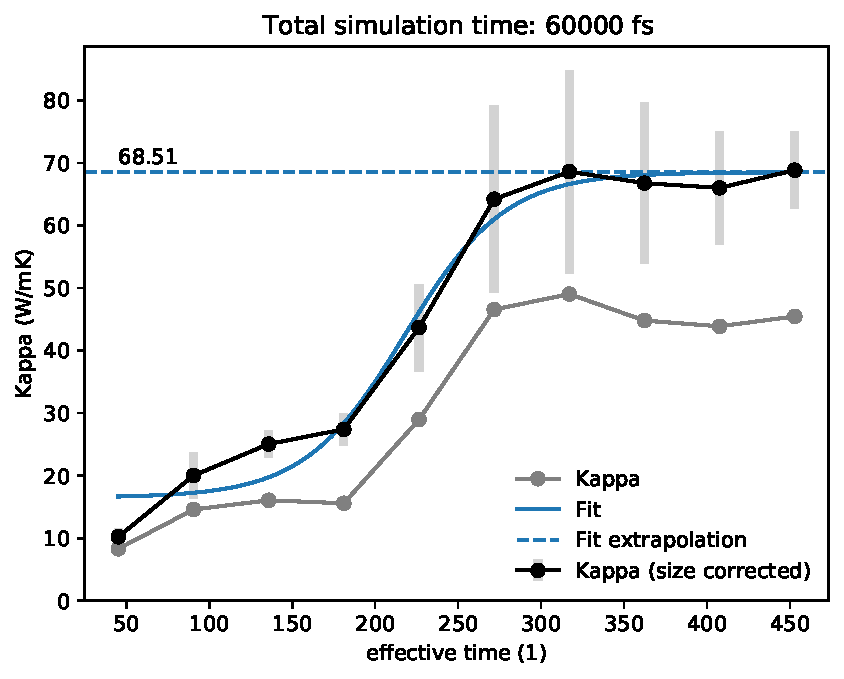
\includegraphics[width=\textwidth]{./data/plots/kappa_convergence/examples/225_MgO.pdf}
	\caption{Thermal conductivity $\kappa$ as function of the effective simulation time $\teff = 7.5\,{\rm THz} \cdot t_0$ as defined in Eq.\,\ref{eq:imp.teff}. Values are given as the ensemble average over three independent trajectories. The error bars are computed according to Eq.\,\eqref{eq:imp.kappa.err} as the standard error of the ensemble average. The blue curve is a logistic curve defined in Eq.\,\eqref{eq:imp.f_logistic} fitted to the $\kappa$ values, the dashed blue curve is the infinite time limit of the fitted function. Gray dots represent the thermal conductivity as given by the simulation without the size-correction scheme.
	
	Please note that the values for $\kappa$ shown here cannot be directly compared to the value displayed in Fig.\,\ref{fig:imp.hfacf.kappa.1} or \ref{fig:imp.kappa.bte.correction}, because the latter only show single components of single runs, which can vary substantially from the total average.
	\mscomment{x-label: teff}
	}
	\label{fig:imp.kappa.convergence.MgO}
\end{figure}
The convergence of the scalar thermal conductivity is shown in Fig.\,\ref{fig:imp.kappa.convergence.MgO} as function of a dimensionless \emph{effective simulation time} $t_0^{\rm eff}$, which we define via
\begin{align}
	\teff = t_0 \cdot \bar{\omega}_{\rm min}~,
	\label{eq:imp.teff}
\end{align}
where $t_0$ is the (truncated) simulation time, and $\bar{\omega}_{\rm min}$ is a characteristic frequency for the slow degrees of freedom of the system, chosen as the mean frequency of the lowest 20\,\% of the vibrational spectrum as explained in Fig.\,\ref{fig:imp.w_eff}. In MgO, this frequency is 7.5\,THz.
\begin{marginfigure}
	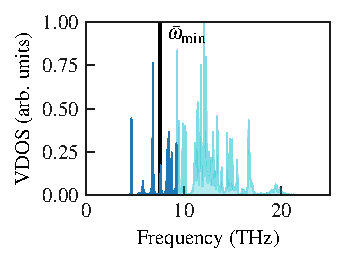
\includegraphics[width=\textwidth]{./data/plots/kappa_convergence/t_eff/vdos.pdf}
	\caption{Vibrational density of states (VDOS) for MgO. Light blue is the entire VDOS, solid blue is the lowest 20\,\% of the spectrum. $\bar{\omega}_{\rm min}$ is calculated as the average frequency in the low part of the spectrum.}
	\label{fig:imp.w_eff}
\end{marginfigure}
Figure~\ref{fig:imp.kappa.convergence.MgO} shows that the thermal conductivity converges after an effective simulation time of $\teff \approx 300$, which corresponds to a time of 40\,ps, where the value of $\kappa$ reaches a plateau within the error bars. The overall shape of the curve can be described as follows: Simulations shorter than 20\,ps ($\teff \lesssim 150$) sample the early decay of the HFACF which contribute about 30\,W/mK to the total thermal condcutivity. After a simulation time of 25\,ps ($\teff \gtrsim 190$), the late decay of the HFACF is sampled, contributing more than double the amount to the total thermal conductivity of $68.8 \pm 6.1$\,W/mK after the total simulation time. In the plot, this two-step behavior is approximated by a logistic function 
\begin{align}
	f(t) 
		= \frac{L}{1 + \exp \left(-\frac{(t-t_{\rm inflection})}{\tau} \right)} + f_0~,
	\label{eq:imp.f_logistic}
\end{align}
which allows to accurately quantify the simulation times where the second super-linear increase in $\kappa$ occurs,~i.\,e.,~the region in the vicinity of the inflection point located at $t_{\rm inflection} = 218$, which corresponds to a simulation time of 29\,ps.
%The plot also shows the thermal conductivities obtained without the finite-size correction discussed earlier as gray dots. Without this correction, the final value would be $45.5 \pm 6.1$\,W/mK. The finite-size correction therefore increases this value by about 50\,\%.

\section{Comparison to Literature Values}
\label{sec:mgo.experiments}
Periclase MgO is an important constituent of the earth mantle and its thermal properties have been studied in detail both experimentally and theoretically~\cite{Charvat.1957,Slack.1962,touloukian1970,Macpherson.1983,Koker.2009,Stackhouse.2010,Tang.2010,Dekura.2017}. We list the common experimental reference values for the thermal conductivity of periclase MgO in Tab.\,\ref{tab:exp.MgO}.
\begin{table}[ht]
  \centering
  \fontfamily{ppl}\selectfont
  \begin{tabular}{lc}
    \toprule
    Reference & Thermal conductivity \\
    & at 300\,K (W/mK) \\
    \midrule
    Slack~1962~\cite{Slack.1962} & $59.7$ \\
    Touloukian et al.~1970~\cite{touloukian1970} & $59.8$ \\
    MacPherson and Schloessin~1983~\cite{Macpherson.1983} & $61.7 \pm 10.5$ \\
    Andersson and B\"ackstr\"om~1986~\cite{Andersson.1986} & $55.2 \pm 0.4$ \\
    Katsura 1997~\cite{Katsura.1997} & $65 \pm 15^{\,\dagger}$ \\
    Dalton et al.~2013~\cite{Dalton.2013} & $53 \pm 2$ \\
    Hofmeister~2014~\cite{Hofmeister.2014} & $50.1$ \\
    This work (theory) & $68.8 \pm 6.1$ \\
    \bottomrule
    \vspace{.5em}
  \end{tabular}
  \caption{Experimental values for the thermal conductivity of periclase MgO at ambient conditions. The value marked by $\dagger$ was computed from thermal diffusivity measurements by Katsura according Ref.\,\cite{Hofmeister.2014} with parameters from Ref.~\cite{Dubrovinsky.1997,Chase.1998}.
  }
  \label{tab:exp.MgO}
\end{table}
The aiGK value presented in this work agrees within the statistical precision with the experimental value presented by MacPherson and Schloessin~\cite{Macpherson.1983}. It slightly overestimates the values reported by Slack~\cite{Slack.1962}, Touloukian et al.~\cite{touloukian1970}, and Katsura~\cite{Katsura.1997}. More recent experiments by Dalton et al. and Hofmeister using laser-flash experiments report lower values of thermal conductivity in the range of 50-55\,W/mK~\cite{Dalton.2013,Hofmeister.2014}.

Overall, we overestimate the experimentally observed thermal conductivity by about 10-30\,\%, depending on the reference. This can be explained by two factors: First, the simulation deals with isotopically pure MgO. Isotope scattering is known to decrease the thermal conductivity in MgO by up to 46\,\% when the natural abundance of magnesium isotopes is considered~\cite{Slack.1962,Tang.2010}. As MgO is a major constituent of the earth mantle, available experiments investigate MgO in this form.\footnote{Natural abundance of Mg in the earth mantle is 80\% $^{24}$Mg, 10\% $^{25}$Mg, 10\% $^{26}$Mg~\cite{Berglund.2011}.} Second, the aiGK theory uses classical statistical mechanics, and nuclear quantum effects lowering the heat capacity of MgO and therefore its thermal conductivity are neglected. These effects have been shown to lower the thermal conductivity in MgO by about 5\,\% at 500\,K~\cite{Puligheddu.2019}, a stronger effect can therefore be expected at 300\,K. In total, an overestimation of thermal conductivity in non-isotopically-pure MgO at ambient conditions is therefore expected.\footnote{Unfortunately, experimental measurements for isotopically pure MgO are not available.}
%Furthermore, small imperfections in the simulation tend to increase the thermal conductivity further: The pressure in the aiMD simulation is about 0.5\,GPa, and the thermal conductivity of MgO is known to increase with pressure by up to 6.8\,\% per GPa~\cite{Yukutake.1978}. Also the temperatures observed during the three aiMD runs are, on average, slightly lower than 300\,K.~\footnote{Observed temperatures in the three trajectories: 307.1\,K, 290.7\,K, 286.5\,K.}

We also compare to theoretical values listed in Tab.\,\ref{tab:theo.MgO}.
%
\begin{table}[ht]
  \centering
  \fontfamily{ppl}\selectfont
  \begin{tabular}{lc}
    \toprule
    Reference & Thermal conductivity \\
    & at at 300\,K (W/mK) \\
    \midrule
    de Koker 2010 (LDA)~\cite{Koker.2010} & $\approx 75^{\,\dagger}$ \\
    Stackhouse et al. 2010 (LDA)~\cite{Stackhouse.2010} & $58 \pm 6^{\,\dagger}$ \\
    Tang and Dong 2010 (LDA)~\cite{Tang.2010} & $\approx 66$ \\
    Dekura and Tsuchiya 2017 (LDA)~\cite{Dekura.2017} & $\approx 54$ \\
    Plata et al.~2017 (PBE)~\cite{AAPL} & $54.06$ \\
    Xia et al.~2020 (PBE)~\cite{Xia.2020} & $50.1-58.7$ \\
    This work & $68.8 \pm 6.1$ \\
    \bottomrule
    \vspace{.5em}
  \end{tabular}
  \caption{Theoretical values for the thermal conductivity of periclase MgO at ambient conditions. All cited approaches use a perturbative Boltzmann transport approach with three phonon scattering. Xia and coworkers use three different flavors of Boltzmann transport theory and therefore give three values for thermal conductivity in the indicated range. Values marked with $\dagger$ are extrapolated values using data from higher temperatures using Eq.\,(17) in Ref.\,\cite{Koker.2010} and Eq.\,(5) in Ref.\,\cite{Stackhouse.2010}, respectively. See also discussion in Ref.\,\cite{Haigis.2012}.}
  \label{tab:theo.MgO}
\end{table}
%
Our study agrees well with the values reported by de Koker, and Stackhouse and coworkers~\cite{Koker.2009,Stackhouse.2010}. Both use non-perturbative \emph{ab initio} molecular dynamics-based methods and simulate isotopically pure MgO, they are therefore closely related from a methodological point of view. All other approaches are based on Boltzmann transport theory and account for isotope scattering. They are therefore smaller, overall by about 10-15\,W/mK, and mutually agree quite well irrespective of the xc-functional. The only exception is the value reported by Tang and Dong, which is about 20\,\% larger, which they partially attribute to underestimated lattice constants due to their LDA functional~\cite{Tang.2010}.\footnote{Indeed, Tang and Dong find a density of MgO at ambient conditions of 3.70\,g/cm$^3$, compared with an experimantal value of 3.58\,g/cm$^3$~\cite{Speziale.2001}.}

\newthought{In summary, the agreement with literature values can be considered satisfactory}, in particular with the related computational approaches by de Koker, and Stackhouse and coworkers. In comparison to the experimental literature, we observe a systematic overestimation of available values, which is to be expected due to the lack of isotope effects in our simulations, as discussed.

%Given the wide spread of experimental values in the range of 50--62\,W/mK for non-defect-free MgO samples, and noticing that MgO is not fully classical at 300\,K. Furthermore, please note that MgO is largely harmonic with $\sigmaA = 0.17$ and therefore not an ideally suited candidate material for Green-Kubo studies, as all requirements for perturbative Boltzmann transport are fulfilled, and good quantitative agreement can be achieved with that approach,~cf.~Tab.\,\ref{tab:theo.MgO}.

%\mscomment{no reason to use isotopically pure MgO, add information which istope abundance was used}
%\FK{natural abundance of Mg is 79\% $^{24}$Mg, 10\% $^{25}$Mg, 10\% $^{26}$Mg~\cite{Berglund.2011}, we have approx. 100 Mg atoms in the simulation -> nice project.}
%\mscomment{isotope effect estimation can be improved}
%\FK{True, see discussion in \cite{Haigis.2012} using Eq. (1) from \cite{Tang.2010}.}
%\ADD{Stackhouse \cite{Stackhouse.2010} and Koker \cite{Koker.2009} as discussed in Haigis \cite{Haigis.2012}.}
%\mscorrect{...not ideally suited...: this should be ideal because BT works}
%\FK{yes but GK is expensive and isotope scattering + NQE, which are important here, are easier to incorporate into BT}
%\mscomment{Do TangDong use PBEsol or similar?}
%\FK{they use LDA}


\section{Case Study Copper Iodide}

After discussing our implementation of the aiGK method and found reasonable agreement with literature values for periclase MgO,
\mscomment{You should agree if there are no other approximation}
\FK{I listed the most important approximations, for full agreement one would need a consistent comparison with same computational parameters and good statistics, see \cite{Puligheddu.2019}.}
we apply the presented methodology to zincblende copper iodide ($\gamma$-CuI), also know as marshite. CuI is a transparent semiconductor which shows several interesting electronic and thermal transport properties: In particular, its room temperature thermal conductivity is very low with only 1.68\,W/mK~\cite{perry2016}, which is typical for copper halide materials~\cite{Slack.1982}. In polycrystalline thin films, even lower thermal conductivities of 0.48--0.55\,W/mK have been reported~\cite{Yang.2017,Coroa.2019}.

In our initial screening for anharmonic materials, CuI was detected as particularly anharmonic, with a one-shot $\sigmaAOS = 0.37$, 
\mscorrect{0.4 ist mild}
\FK{no.}
and a value of $\sigmaA = 0.4-0.5$ in molecular dynamics simulations. The peculiar dynamical effects occuring in CuI,~.i.\,e.,~formation of metastable Cu defects below the superionic phase transition, have been discussed in Sec.\,\ref{sec:defects.CuI} in the previous chapter. CuI can therefore be considered a bigger challenge for dynamical simulations compared to MgO.
\mscomment{I disagree, CuI should be easier for GK}
\FK{yes, for GK, but I meant common ab initio simulations in general. Clarify}



\subsection{Thermal conductivity}
Following the same recipe presented earlier in this chapter, the convergence of the aiGK thermal conductivity with effective simulation time is shown in Fig.\,\ref{fig:imp.kappa.convergence.CuI} for CuI at room temperature.
\begin{figure}
	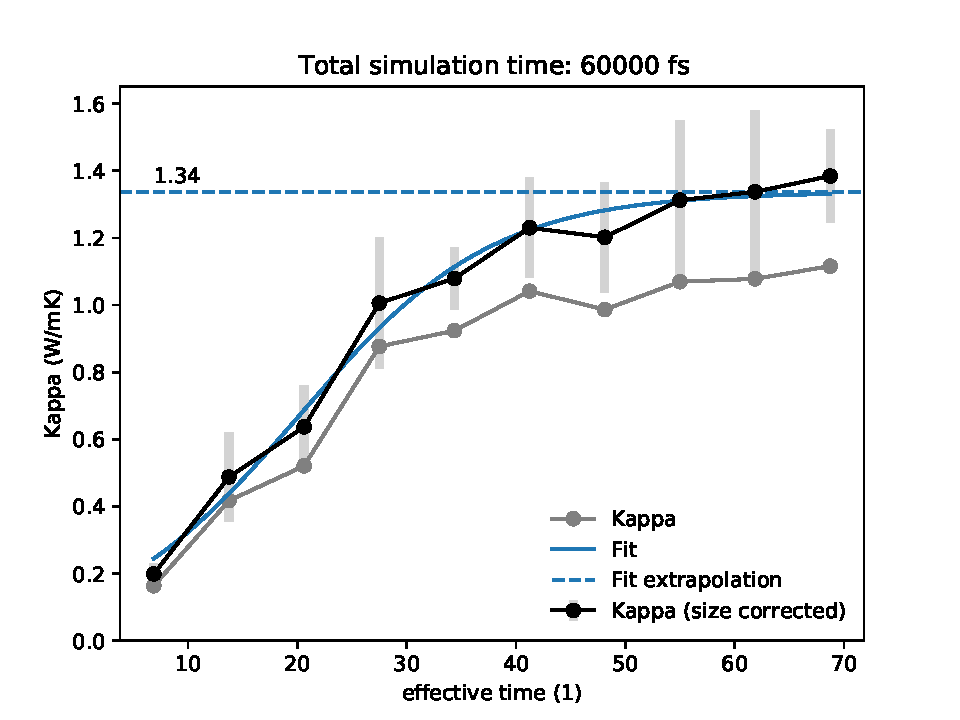
\includegraphics[width=\textwidth]{./data/plots/kappa_convergence/examples/216_CuI.pdf}
	\caption{Thermal conductivity $\kappa$ as function of the effective simulation time $\teff = 1.1\,{\rm THz} \cdot t_0$ as defined in Eq.\,\ref{eq:imp.teff}. Values are given as the ensemble average over three independent trajectories. The error bars are computed according to Eq.\,\eqref{eq:imp.kappa.err} as the standard error of the ensemble average. The blue curve is a logistic curve defined in Eq.\,\eqref{eq:imp.f_logistic} fitted to the $\kappa$ values, the dashed blue curve is the infinite time limit of the fitted function. Gray dots represent the thermal conductivity as given by the simulation without the size-correction scheme.
}
	\label{fig:imp.kappa.convergence.CuI}
\end{figure}
The final value of $1.38 \pm 0.14$\,W/mK is approached within error bars after an effective simulation time of $\teff = 40$, which corresponds to $t_0=36$\,ps. The finite size correction contributes about 0.26\,W/mK to the thermal conductivity,~i.\,e.,~19\,\% of the total value.

Comparing this to the available literature in Tab.\,\ref{tab:exp.CuI}, we find good agreement with the  experimental reference value of 1.68\,W/mK, while the value is clearly above the thin-film limit of 0.55\,W/mK.
\begin{table}[ht]
  \centering
  \fontfamily{ppl}\selectfont
  \begin{tabular}{lc}
    \toprule
    Reference & Thermal conductivity \\
    & at 300\,K (W/mK) \\
    \midrule
    CRC Handbook~\cite{perry2016} (experiment) & 1.68 \\
    Yang et al.~\cite{Yang.2017} (experiment) &  0.55$^{\,\dagger}$ \\
    Togo et al.~\cite{phono3py} (theory) & 6.55--7.22 \\
    This work & $1.38 \pm 0.14$ \\
    \bottomrule
    \vspace{.5em}
  \end{tabular}
  \caption{Experimental values and one theoretical reference for the thermal conductivity of marshite CuI at ambient conditions. The value from Yang et al. marked by $\dagger$ is from a thin film experiment, and therefore can be regarded as a lower bound of the bulk thermal conducitivity~\cite{Yang.2017}.}
  \label{tab:exp.CuI}
\end{table}
The theoretical reference on the other hand drastically overestimates the thermal conductivity by a factor of $\approx 4$~\cite{phono3py}. 
\mscomment{Explain in more detail, are there empirical parameters:}
Since the theoretical reference uses a perturbative approach in terms of third-order force constants obtained at the local minimum of the potential-energy surface, a probable explanation for this strong discrepancy is the inability of this approach to model the actual, strongly anharmonic dynamics of CuI with sufficient accuracy. As discussed in Sec.\,\ref{sec:defects.CuI}, CuI inhibits effects like metastable defects, which are qualitatively different from the phonon picture of atoms moving about a well defined reference position in a nearly harmonic potential. These effects are, however, naturally included in the non-perturbative aiGK formalism.


\section{Conclusion}
We have introduced the technical details of our aiGK implementation, and discussed two benchmark systems at ambient conditions: Periclase MgO, and marshite CuI. Although both structures are very simple cubic structures with two atoms in the unit cell, they behave quite differently from a dynamical point of view: MgO is a largely harmonic system which can be regarded as a textbook example for phonon theory, where all basic assumptions hold. In particular there are well defined reference positions, and the deviation from perfectly harmonic interactions is quite weak, with a $\sigmaA = 0.17$ signaling an anharmonic contribution to the forces of about 17\,\%. CuI on the other hand is strongly anharmonic, with $\sigmaA \approx 0.4-0.5$, and displays spontaneous formation of metastable insterstial defects as discussed in Sec.\,\ref{sec:defects.CuI}. 
While perturbative approaches proved to be very accurate for MgO, and even had some advantages compared to aiGK in situations where the material of interest is not fully classical, or isotope scattering lowers the thermal conductivity substantially, the differences were much bigger for the strongly anharmonic CuI, where the perturbative approach overestimated the thermal conductivity drastically, whereas the aiGK is in good agreement.
\mscorrect{When you compare GK with BT you should use same isotope concentration}
\FK{I do, for the simulation. BT includes isotope scattering perturbatively in the postprocessing. We cannot do this. Then what do we compare?}

\mscomment{say that this was the motivation which we could confirm:}
\newthought{The aiGK method is therefore our method of choice} for the investigation of the strongly anharmonic candidate thermal insulators suggested in Chp.\,\ref{chp:anharmonicity} with potentially low thermal conductivity.

\mscorrect{ZP effects should be estimated}
\FK{I do this to some extent later for LiF, and I think available techniques are unsatisfactory.}
\mscorrect{discuss isotope scattering in more detail, in particular w.r.t to harmonic/anharmonic materials}
\FK{I think I did this, clarify.}